\section{Experiment 3 : More Explainable Models}
The results from the previous experiment show that deeper architectures improves explanation quality, in other words, they are more explainable. However, there are some cases that the purposed architectures fail to distribute relevance properly.  Hence, this experiment aims to extend the proposed architectures further to address the problem. We consider the same setting as described in Section \ref{sec:exp2_prob_formulate}. In the following, we are going to describe 3 improvement proposals, namely stationary dropout, LSTM-type architecture,  and lateral connections of convolutional layers.


\subsection{Proposal 1 :  Stationary Dropout}
Dropout is a simple regularization technique that randomly suspends the activity of neurons during the training process\citep{SrivastavaDropoutSimpleWay2014} . This randomized suspension allows the neurons to learn better representations and reduces the chance of overfitting.  As a result, it directly influences the quality of explanation. 

%\addfigure{\ref{fig:lenet_various_dropout}} shows explanations of LeNet trained with different dropout probability.

%\begin{figure}[!htb]
%\centering
%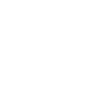
\includegraphics[draft,width=0.5\textwidth]{/sketch/placeholder}
%\caption{LeNet with various dropout values} 
%\label{fig:lenet_various_dropout}  
%\end{figure}



\begin{figure}[!htb]
\centering
\subfloat[Naive Dropout]{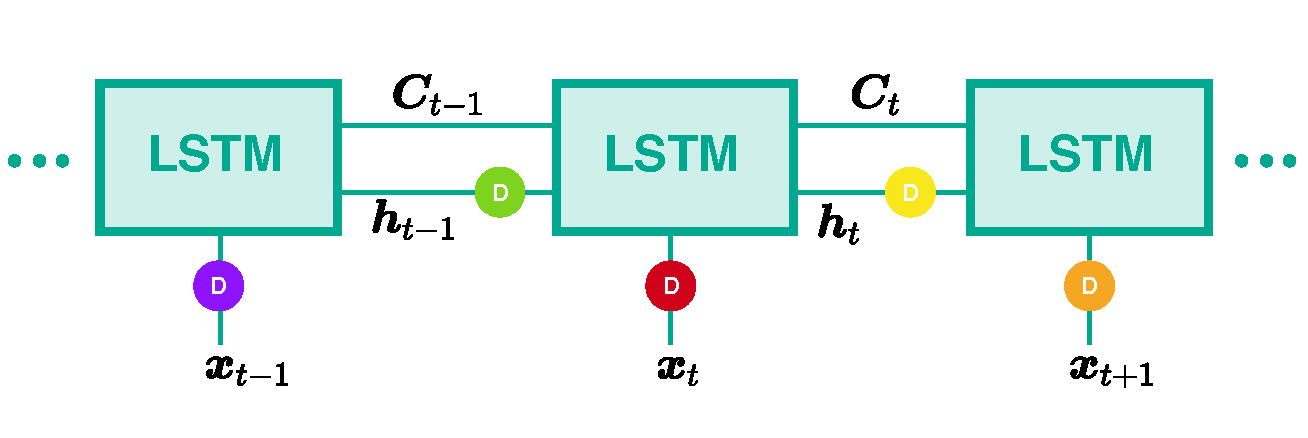
\includegraphics[width=0.45\textwidth]{sketch/lstm_naive_dropout} \label{fig:lstm_naive_dropout}} 
\subfloat[Stationary Dropout]{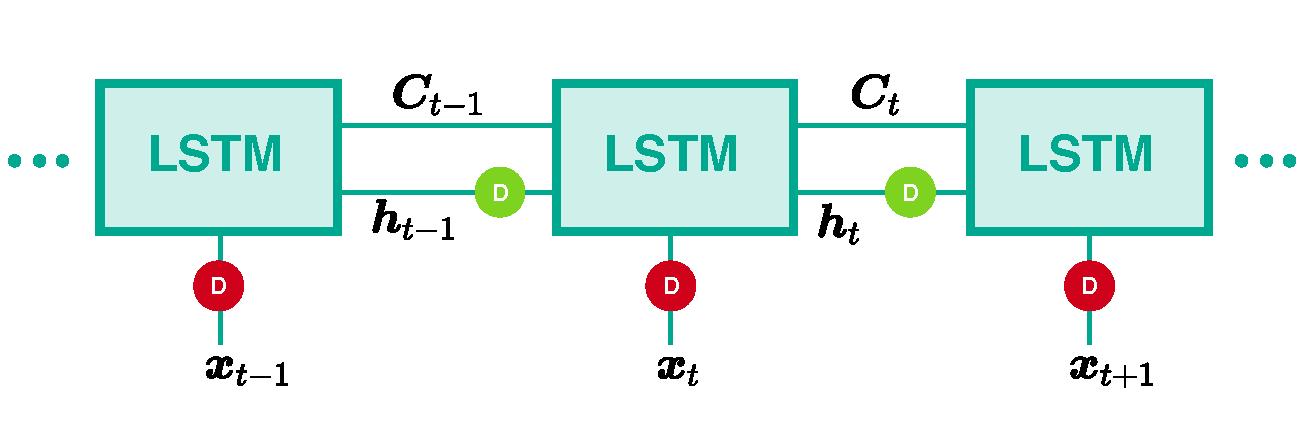
\includegraphics[width=0.45\textwidth]{sketch/lstm_variational_dropout} \label{fig:lstm_variational_dropout}}

\patcaption{LSTM with different dropout approaches.}{\textcircled{\tiny \textbf D} indicates a dropout mask and its color represents a suspension activity.}
\label{fig:dropout_lstm}
\end{figure}

Unlike typical feedforward architectures, layers in RNN are shared and reused across input sequence. A question arises whether the same neurons in those layers should be suspended or they should be different ones. \addfigure{\ref{fig:dropout_lstm}} illustrates these two different approaches where different colors represent different dropping activities. In particular, \citet{GalTheoreticallyGroundedApplication2016} proposed and demonstrated that training LSTM and GRU with this stationary dropout approach on language modeling tasks improved the performance of the models.

%this stationary dropout was first proposed by \citet{GalTheoreticallyGroundedApplication2016} who applied  the technique to LSTM and GRU and found accuracy improvements on language modeling tasks.

\subsection{Proposal 2 : LSTM-type architecture}
\begin{figure}[!htb]
\centering
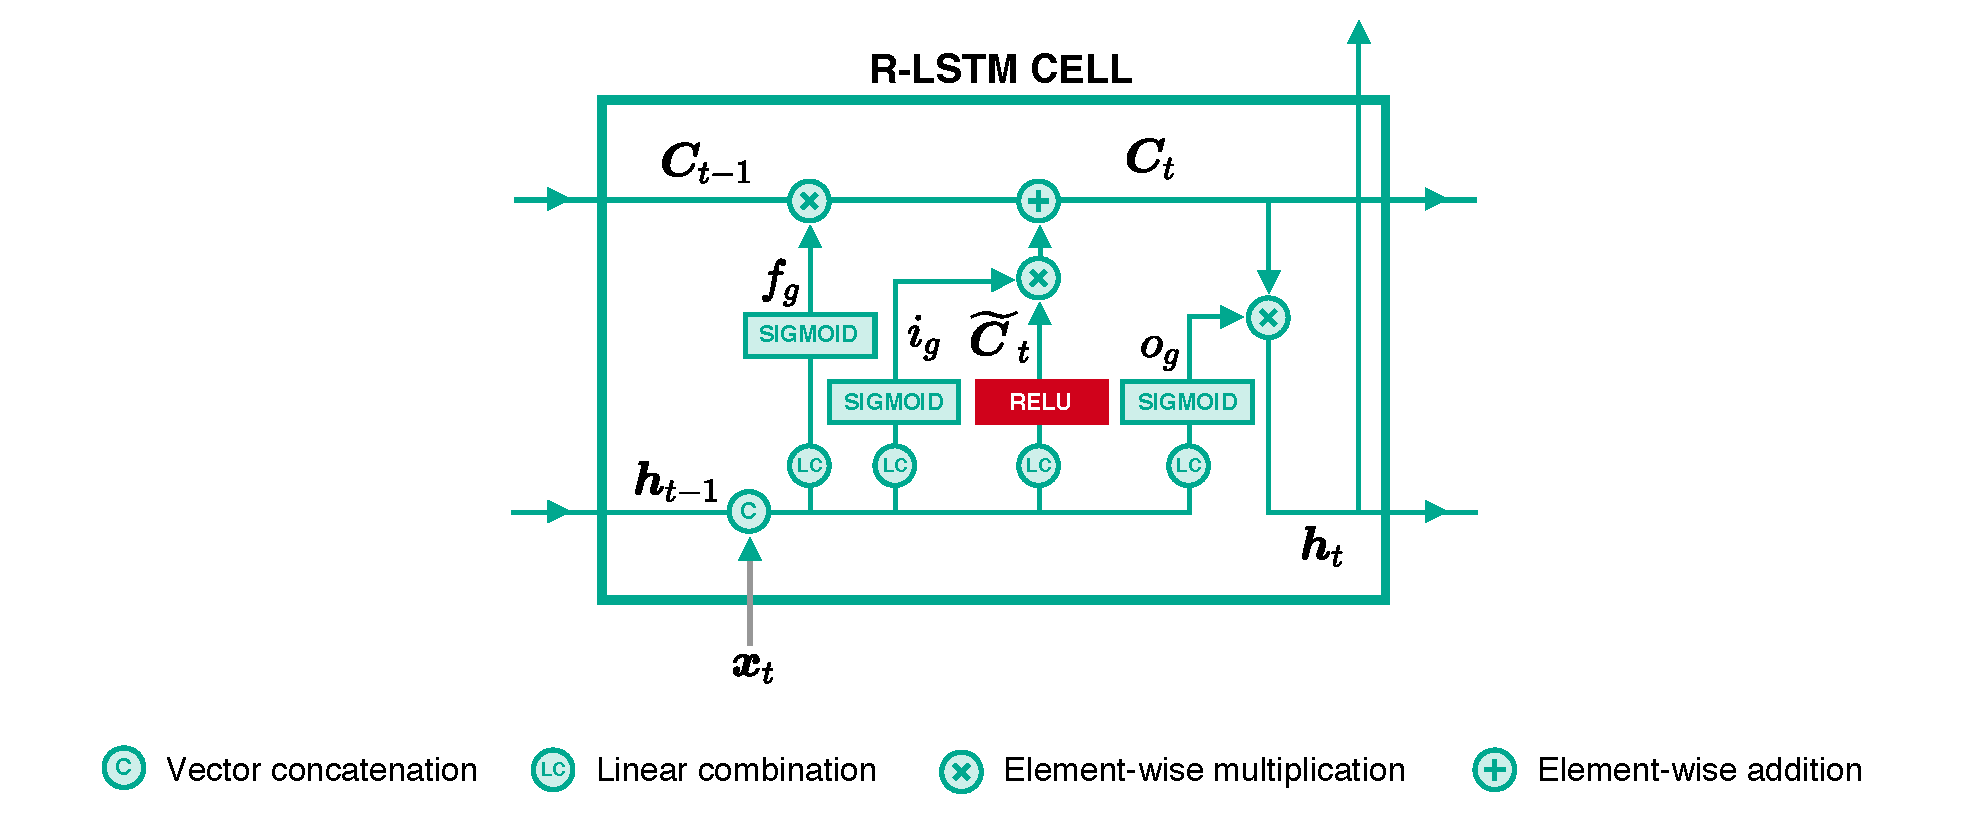
\includegraphics[width=\textwidth]{sketch/relu_lstm}
\caption{R-LSTM Structure} 

\label{fig:relu_lstm} 
\end{figure}

It is already shown that gating units and addictive updates are critical mechanisms that enable LSTM to learn long-term dependencies efficiently \citep{GreffLSTMsearchspace2017, JozefowiczEmpiricalExplorationRecurrent2015}. However, LSTM is not readily applicable to explanation methods we are considering, except only SA. More precisely, the use of sigmoid and tanh activations violates the assumption of GB and DTD. Therefore, we propose a slightly modified version of LSTM where ReLU activation is used to compute cell state candidate $\widetilde{C}_t$ instead of the tanh function. This results in $C_t \in \mathbb{R}^+$, hence the tanh activation for $h_t$  is also removed.  As suggested in \citep{ArrasExplainingRecurrentNeural2017},  sigmoid activations are treated as constants when applying DTD and LRP. For GB, we propose to set the gradients to zero. We refer this architecture as R-LSTM to differentiate from the original.  \addfigure{\ref{fig:relu_lstm}} presents an overview of R-LSTM architecture.


\subsection{Proposal 3 : Convolutional layer with lateral connections}
We have already seen its contributions from the previous experiments that convolution and pooling operator enable neural networks to learn hierarchical and invariant representations yielding models that have higher accuracy as well as the quality of explanation. However, \rnncell{ConvDeep} architecture we proposed in Section \ref{sec:exp2} does not seem to be capable enough to allocate relevance to the right input in some sequences properly. We suspect that it is because the architecture has recurrent connections only at a fully-connected layer after convolutional and pooling layers. 


 \begin{figure}
\centering
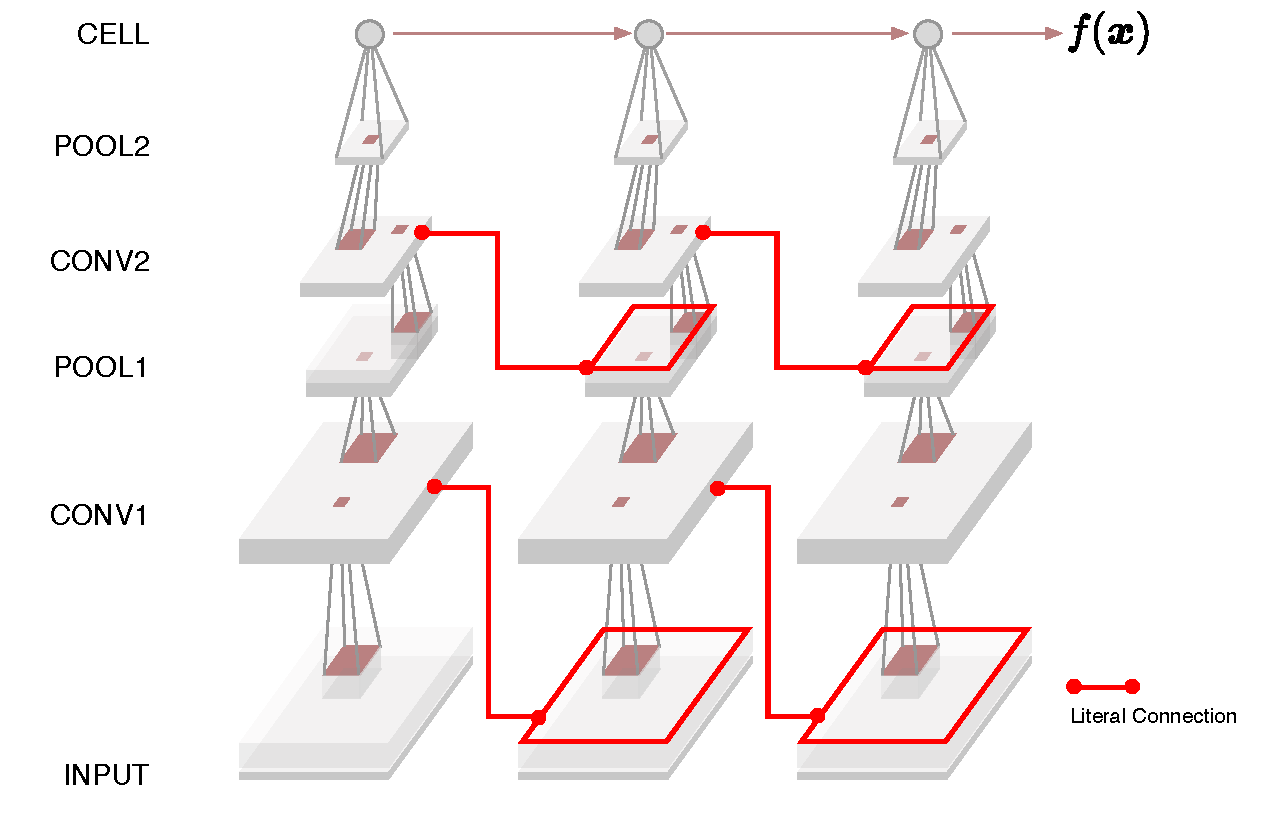
\includegraphics[width=0.9\textwidth]{sketch/conv_literalconn}
\patcaption{ConvDeep with lateral connections (\rnncell{Conv$^+$Deep}).}{} 
\label{fig:conv_literalconn}
\end{figure}

	Therefore, we propose to also add recurrent connections between convolutional operators of each time step. We name these connections as \textit{lateral connections} and \addfigure{\ref{fig:conv_literalconn}} illustrates such connections in red. From the following, we are going to refer Conv$^+$ to the setting that convolutional layers have these  lateral connections.  It is worth noting that these connections are possible only when dimensions of input before and result after convolution are the same.

\subsection{Result}

\begin{figure}
\centering
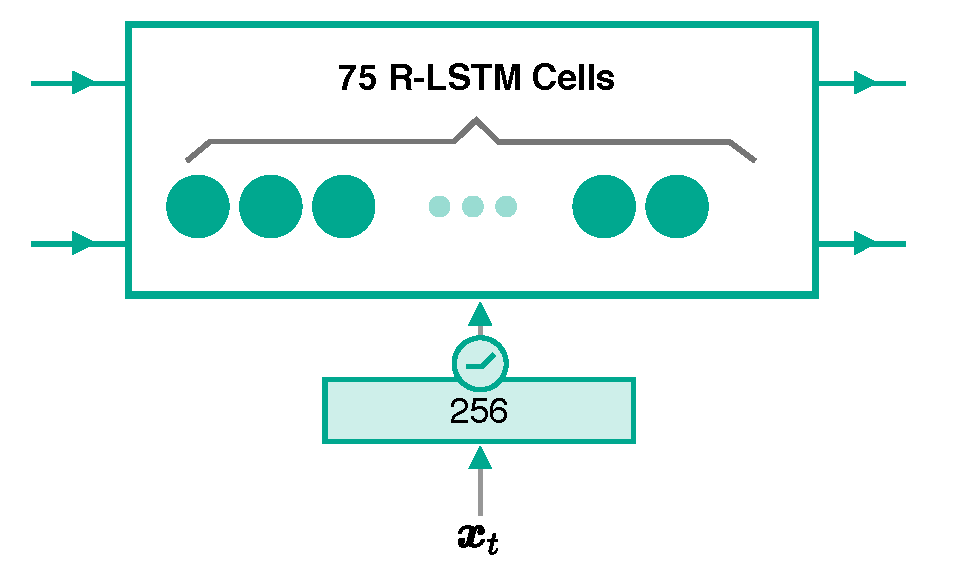
\includegraphics[width=0.5\textwidth]{sketch/r_lstm_setting}
\patcaption{Setting of R-LSTM.}{} 
\label{fig:rlstm_setting}
\end{figure}


We divided this experiment into two parts. The first part focuses on the stationary dropout and R-LSTM proposal. We refer models trained with stationary dropout with $-SD$ suffix. The Deep architecture is used as the baseline.  For R-LSTM's configuration, we also added one fully-connected layer with 256 neurons between the input and 75 R-LSTM cells to make it comparable to the Deep architecture. \addfigure{\ref{fig:rlstm_setting}} visualizes the details.


In the second part, we discuss results from  Conv$^+$ and ConvR-LSTM-SD. The latter architecture is simply R-LSTM-SD that the first fully-connected layer is replaced by convolutions and pooling layers with the same configuration as in ConvDeep. The number of R-LSTM cells is also the same as the first part. Therefore, ConvDeep and R-LSTM-SD are the baseline architectures.


Table \ref{tab:maj_exp3_model_acc} shows the number of trainable parameters in the proposed architectures as well as accuracy.

\renewcommand{\arraystretch}{1.5}
\begin{table}[h]
\begin{center}
\begin{tabular}{lc|c|c|}
\cline{3-4}
& &
\multicolumn{2}{c|}{\parbox{3.5cm}{ \vskip 1mm \centering \textbf{Accuracy} \vskip 1mm}} \\ \hline
\multicolumn{1}{|l|}{\textbf{Cell architecture}} & \textbf{No. variables} & \textbf{MNIST-MAJ} & \textbf{FashionMNIST-MAJ} \\ \hline
\multicolumn{1}{|l|}{Deep-SD}                  & 153,578             & 98.10\% & 89.47\% \\ 
\multicolumn{1}{|l|}{R-LSTM}                    & 145,701   & 98.50\% & 91.35\% \\ 
\multicolumn{1}{|l|}{R-LSTM-SD}              &  145,701                & 98.57\% & 91.52\% \\ 
 \multicolumn{1}{|l|}{Conv$^+$Deep}       & 175,418                 & 97.92\% & 88.10\% \\
 \multicolumn{1}{|l|}{ConvR-LSTM-SD}      & 152,125                 & 99.35\% & 93.60\%  \\ 
\multicolumn{1}{|l|}{Conv$^+$R-LSTM-SD}   & 175,741                & 98.48\% & 88.19\%  \\ \hline 
\end{tabular}

\end{center}
\caption{Number of trainable variables and model accuracy of the  proposed architectures for MNIST-MAJ and FashionMNIST-MAJ.}
\label{tab:maj_exp3_model_acc}
\end{table}
\renewcommand{\arraystretch}{1}

%todo: mention that Deep is from previous result

\subsubsection{Part 1 : Stationary Dropout and R-LSTM}
 \begin{figure}[!htb]
\centering
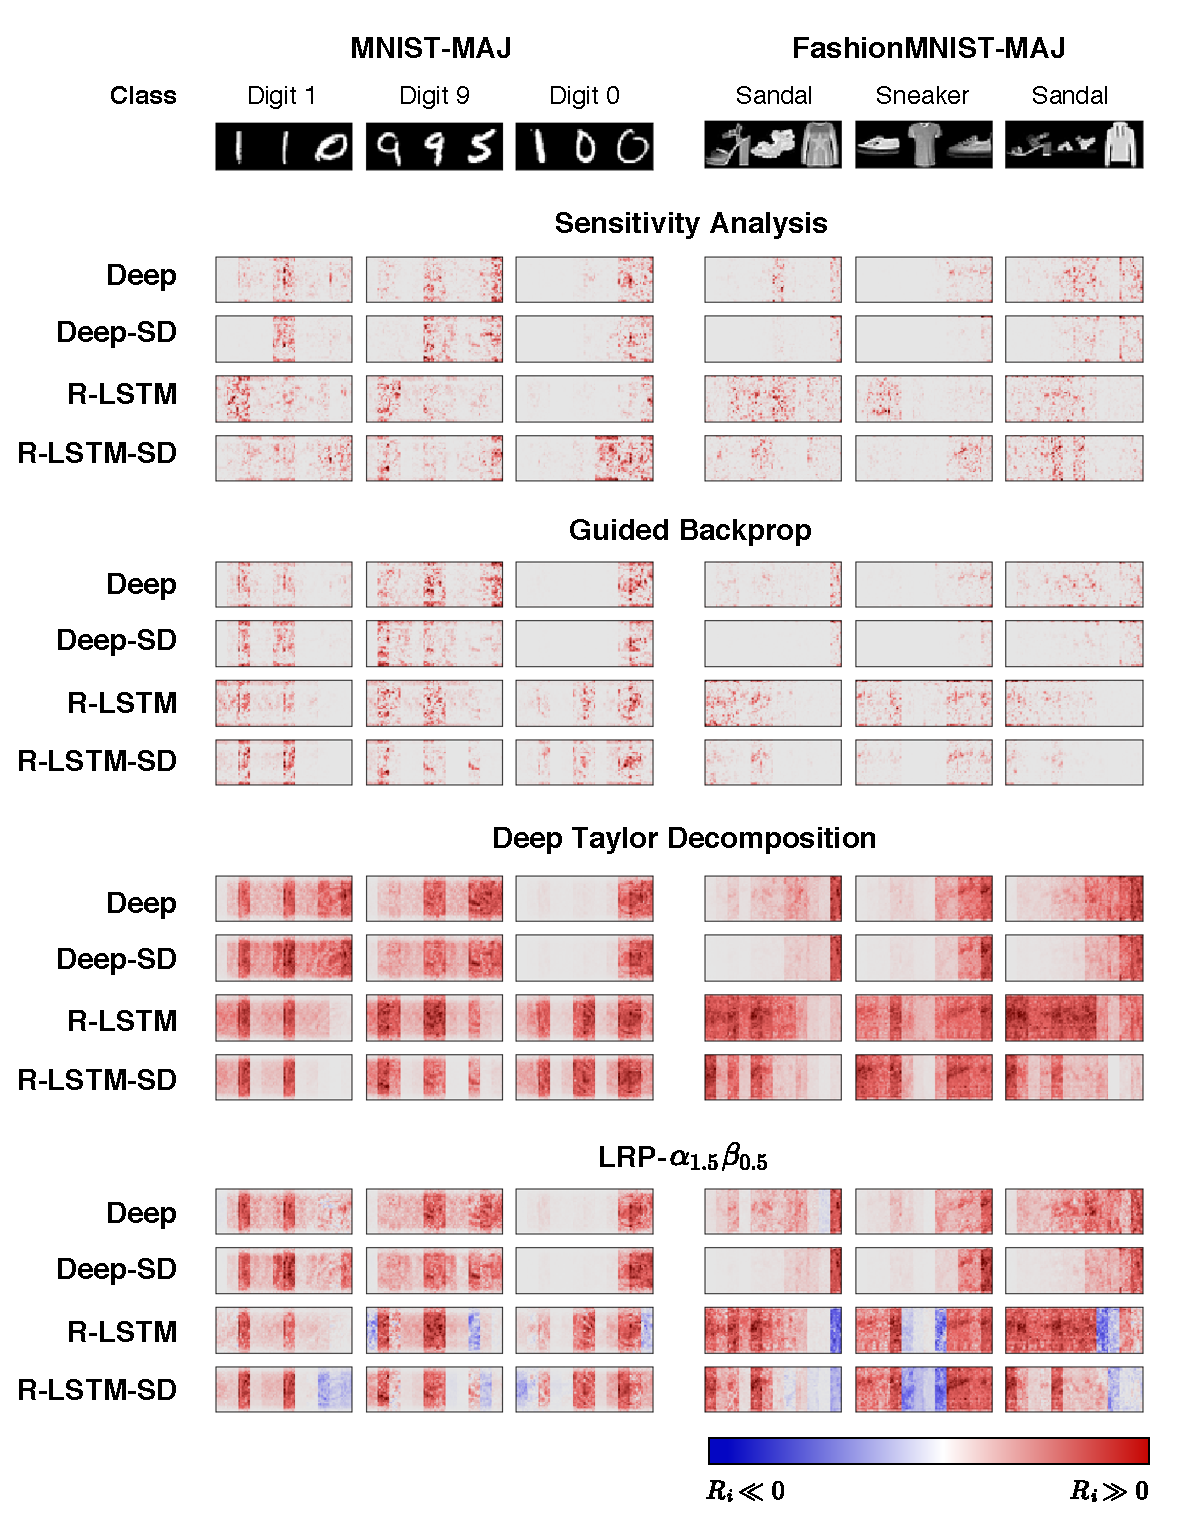
\includegraphics[width=0.8\textwidth]{sketch/heatmap_msc_rlstm_exp}
\patcaption{Relevance heatmaps produced by different explanation techniques on Deep and R-LSTM architecture trained on MNIST-MAJ and FashionMNIST-MAJ with sequence length $T=12$ and different dropout configurations.}{\heatmapscaleexplain} 
\label{fig:heatmap_msc_rlstm_exp}
\end{figure}

\addfigure{\ref{fig:heatmap_msc_rlstm_exp}} shows explanation heatmaps of the first part of this experiment. Here, variants of Deep and R-LSTM are compared. From the figure, it is apparent that R-LSTM provides better explanations than the Deep architecture. We can clearly observe the improvements from GB, DTD and $\lrpp$ heatmaps. Moreover, training with stationary dropout seems to increase explanability of  R-LSTM. This is well notable on DTD and $\lrpp$ explanations. In contrast, the stationary dropout does not seem to have any noticeable impact on the explanations of the Deep architecture.


 \begin{figure}[!htb]
\centering
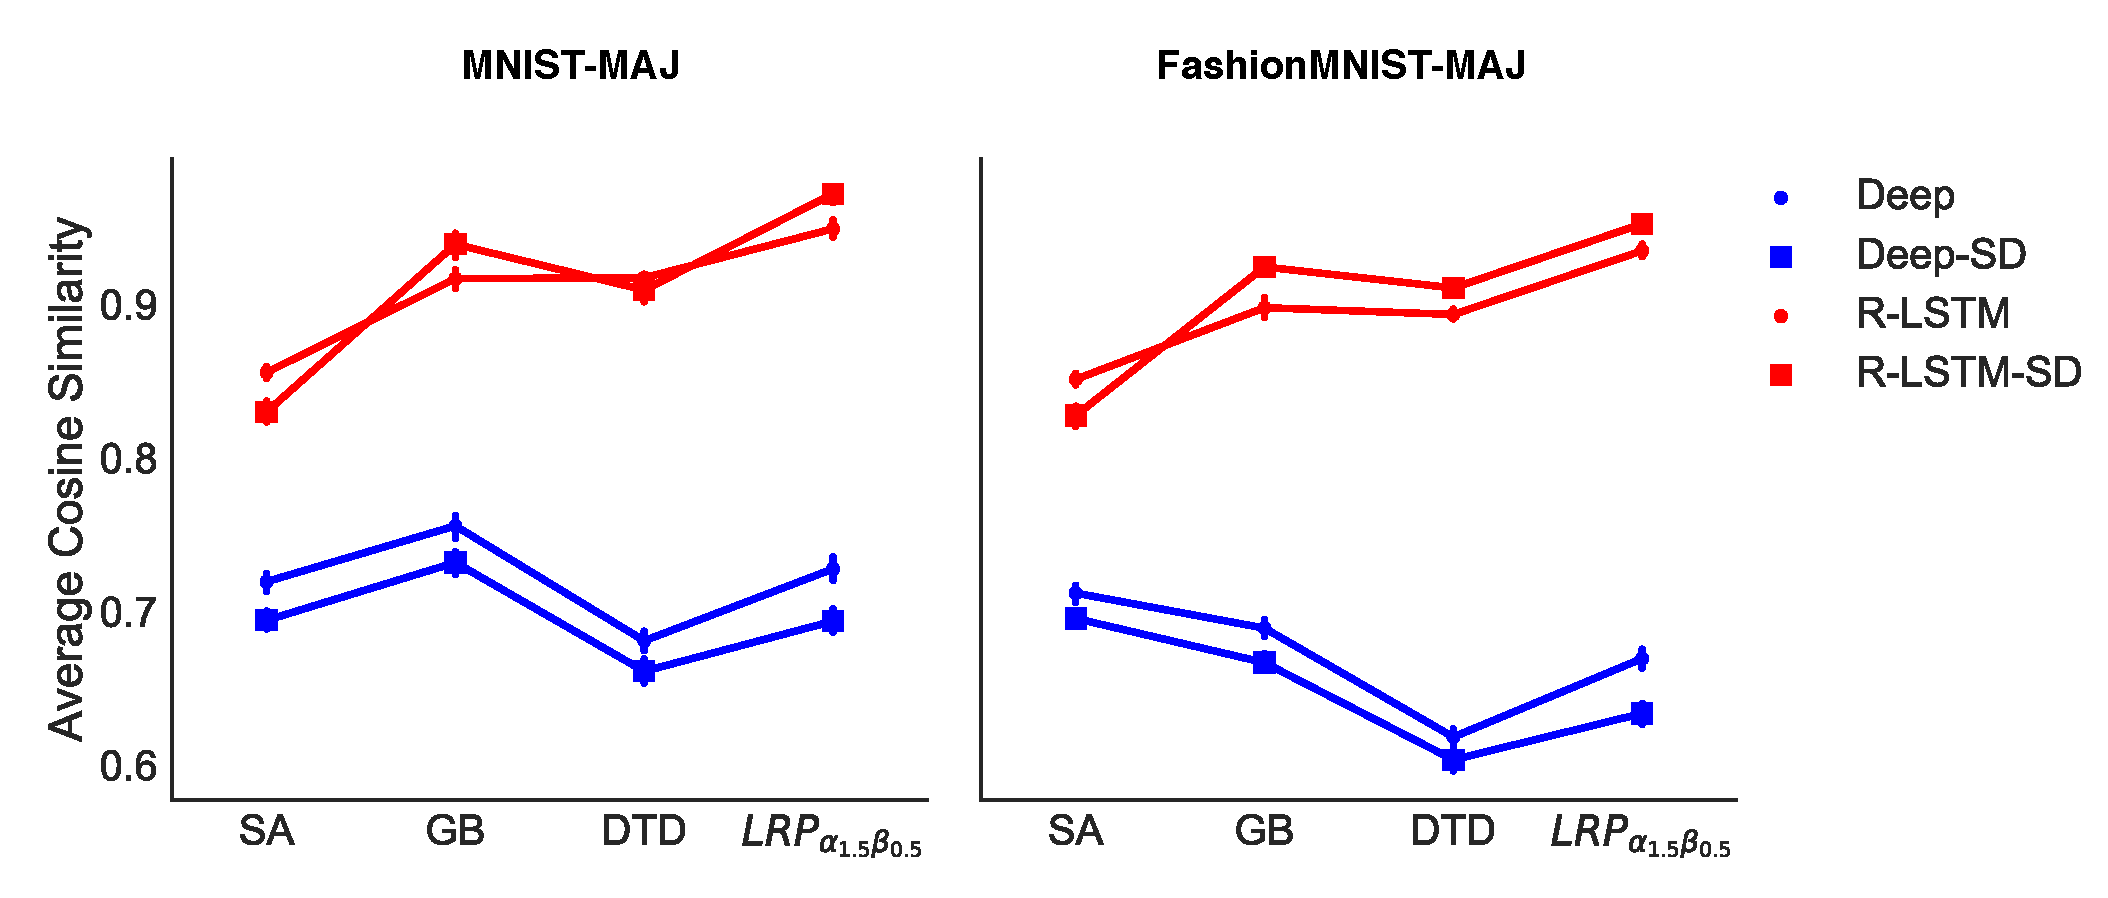
\includegraphics[width=\textwidth]{sketch/rel_dist_rlstm_exp}
%\caption{}  }. 
\patcaption{Average cosine similarity from different explanation techniques on Deep and R-LSTM architecture.}{The baseline is the Deep architecture depicted by dotted blue line. \quantitativeplotexplain}

\label{fig:rel_dist_rlstm_exp}
\end{figure}

\addfigure{\ref{fig:rel_dist_rlstm_exp}} presents quantitative evaluations of the first part. The plots show that the R-LSTM architecture significantly improves relevance distribution than the Deep architecture regardless of explanation techniques.  This means that R-LSTM is more explainable than the Deep architecture. Similar to one of observations in Section \ref{sec:exp1_result}, we also see that the proportion of the improvement of DTD and LRP seem to have a more significant advantage from R-LSTM than the other methods.  

Moreover, \addfigure{\ref{fig:rel_dist_rlstm_exp}}  also shows that  R-LSTM trained with stationary dropout, or R-LSTM-SD, seems to have better explanations than R-LSTM on every method, except SA. On the other hand, this does not seem to be the case for the Deep architecture. In fact, the plots show that the Deep-SD architecture has notably worse results than the Deep architecture.

%This might be due to more heterogeneous structures in FashionMNIST than MNIST samples. Particularly, we believe that  keeping dropout mask the same for all step would benefit the network to  learn such latent features more efficiently. 
%\todo{hypo thesis?}
%\clearpage

%todo mention that ConvDeep, R-LSTM-SD from previous result
\subsubsection{Part 2 : ConvDeep with lateral connections and ConvR-LSTM}
 \begin{figure}[!htb]
\centering
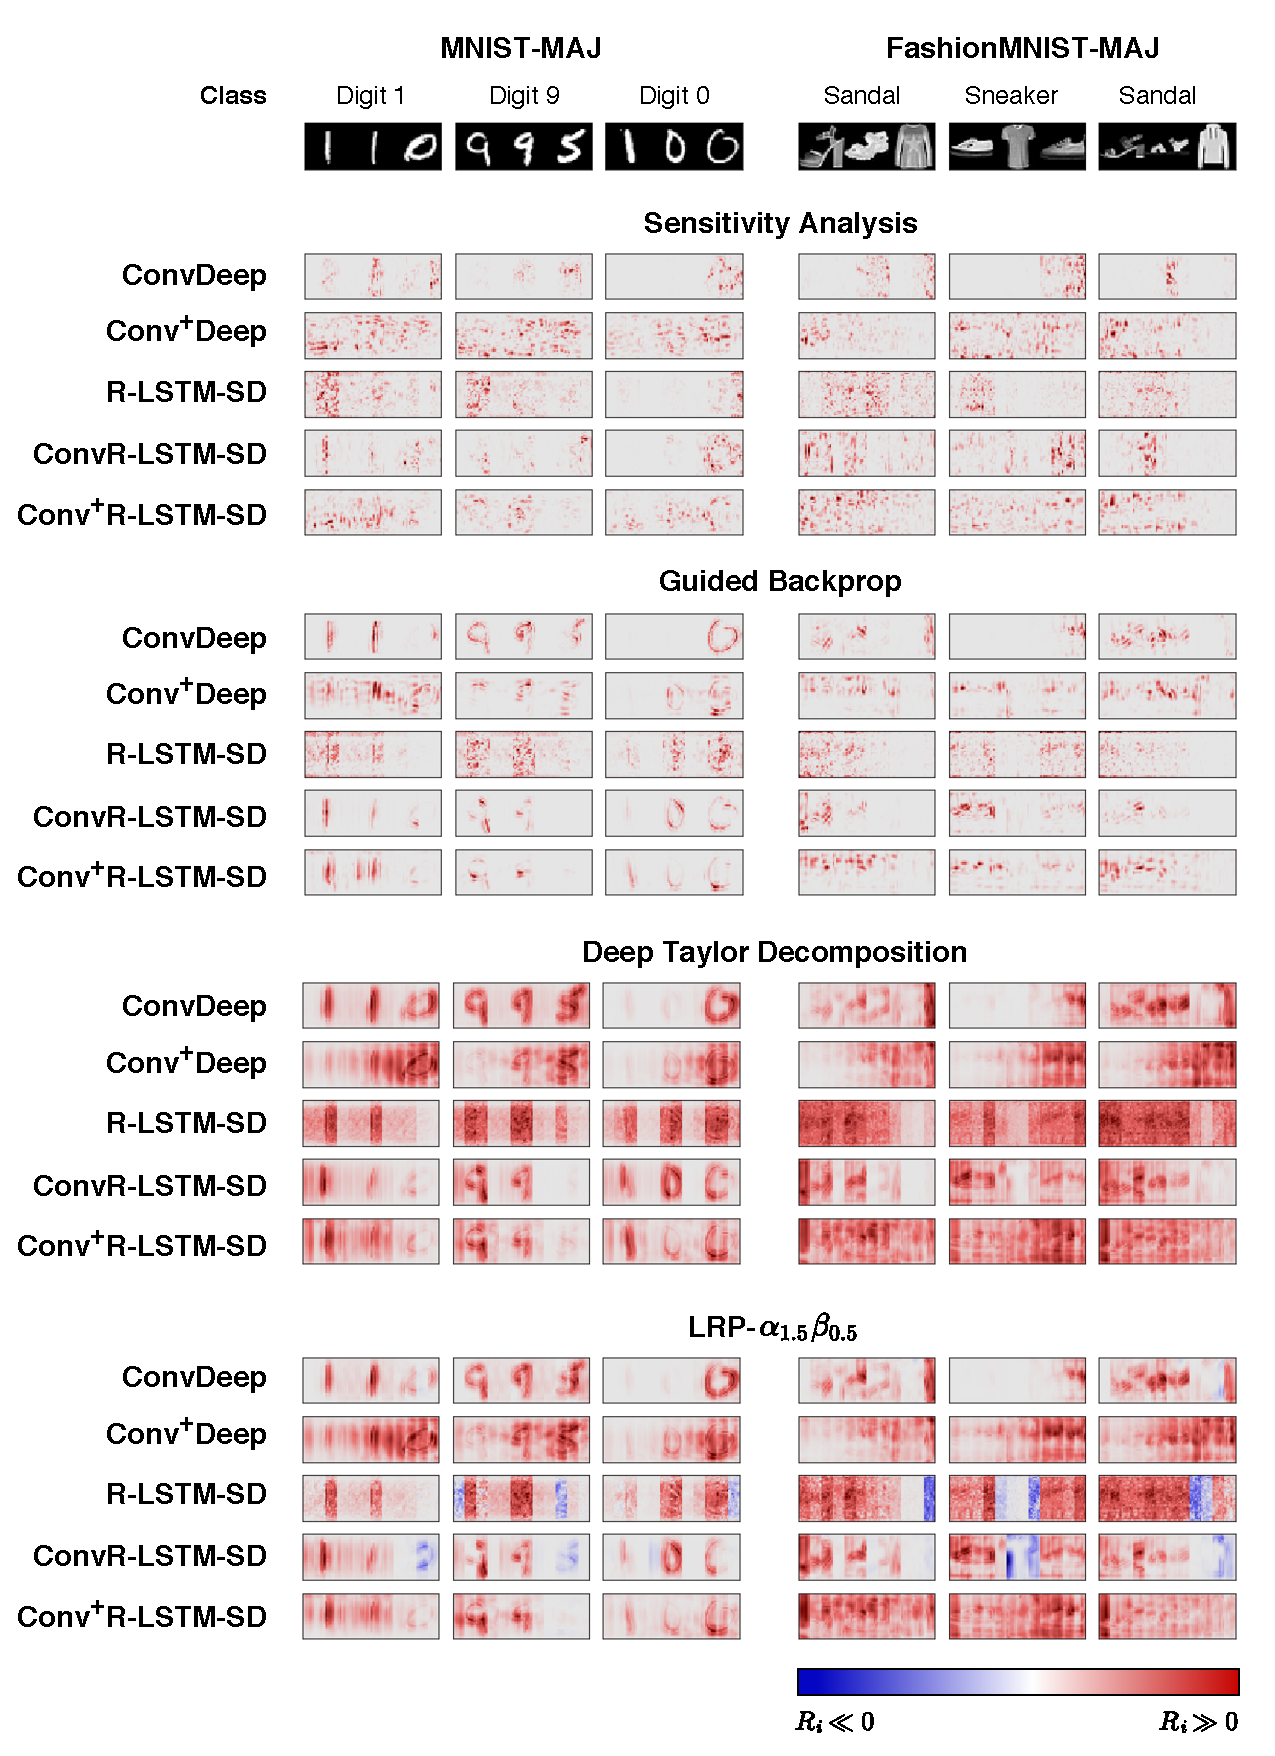
\includegraphics[width=0.8\textwidth]{sketch/heatmap_msc_convtran_exp_v2}
\patcaption{Relevance heatmaps produced by different explanation techniques on variants of ConvDeep and R-LSTM architecture trained on MNIST-MAJ and FashionMNIST-MAJ with sequence length $T=12$.}{\heatmapscaleexplain} 
\label{fig:heatmap_msc_convtran_exp}
\end{figure}
For the second part, we are going to discuss results from the ConvDeep architecture with lateral connections (Conv$^+$Deep), R-LSTM-SD with convolutional layers (ConvR-LSTM-SD) as well as Conv$^+$R-LSTM-SD.

According to \addfigure{\ref{fig:heatmap_msc_convtran_exp}}, Conv$^+$Deep seems to impact on overall explanations negatively. In particular, this problem is prominent on DTD and $\lrpp$ explanations. For example, consider Digit 1 and Digit 9 sample, their relevance scores should not have been distributed to the last digit's block. The figure also shows relevance heatmaps from ConvR-LSTM-SD. Comparing to R-LSTM-SD, having convolutional and pooling layers does improve  the quality of the heatmaps further. In particular, we can see input's structures from the explanations. \addfigure{\ref{fig:heatmap_msc_convrlstm_pos_rel}} also emphasizes the improvement introduced by the convolutional and pooling layers. Here, we plot the relevance heatmaps by using only positive relevance from $\lrpp$. We can see that the explanations of ConvR-LSTM-SD are well highlighted and reveal substantial features of the samples.


%On the other hand, Conv$^+$Deep seems to improve propagation of relevance on SA and GB method slightly: these heatmaps visually contains more relevance in the blocks of the majority digit/item than the ones from the ConvDeep architecture.

%
% This is specially notable on heatmaps from SA  and GB method. Similarly, Conv$^+$Deep also produces worse results for DTD and $\lrpp$, for example consider Digit 1 and Digit 9 sample, where the relevance scores are unnecessarily distributed to the last digit's block. 
%
%>> According to \addfigure{\ref{fig:heatmap_msc_convtran_exp}}, Conv$^+$Deep has more diffuse explanation heatmaps than ConvDeep. This is specially notable on heatmaps from SA  and GB method. Similarly, Conv$^+$Deep also produces worse results for DTD and $\lrpp$, for example consider Digit 1 and Digit 9 sample, where the relevance scores are unnecessarily distributed to the last digit's block. 



 \begin{figure}[!htb]
\centering
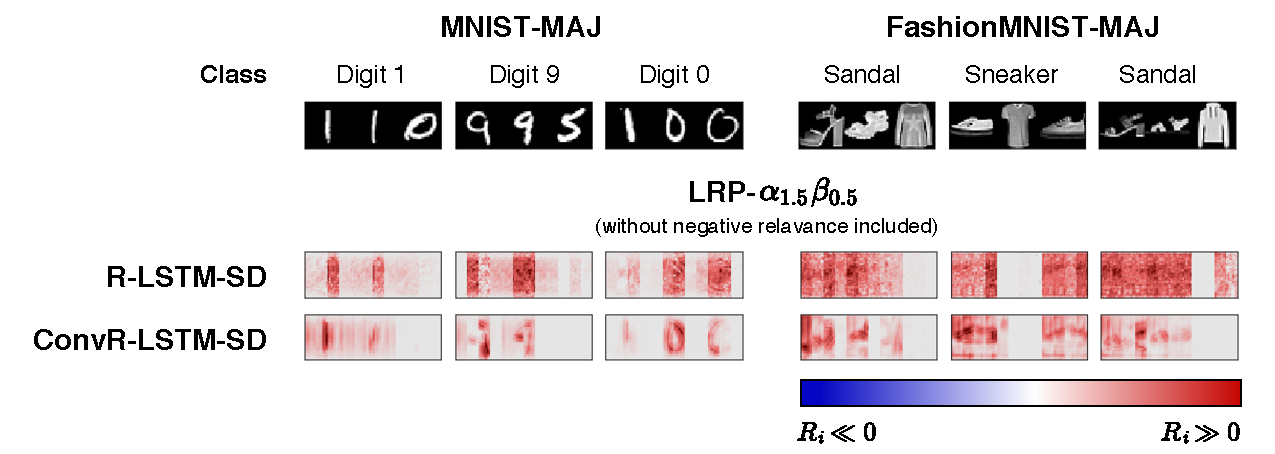
\includegraphics[width=\textwidth]{sketch/heatmap_msc_convrlstm_pos_rel}
\patcaption{Positive relevance heatmaps produced by $\lrpp$ on R-LSTM and ConvR-LSTM architecture trained on MNIST-MAJ and FashionMNIST-MAJ with sequence length $T=12$.}{\heatmapscaleexplain} 
\label{fig:heatmap_msc_convrlstm_pos_rel}
\end{figure}

 \begin{figure}[!htb]
\centering
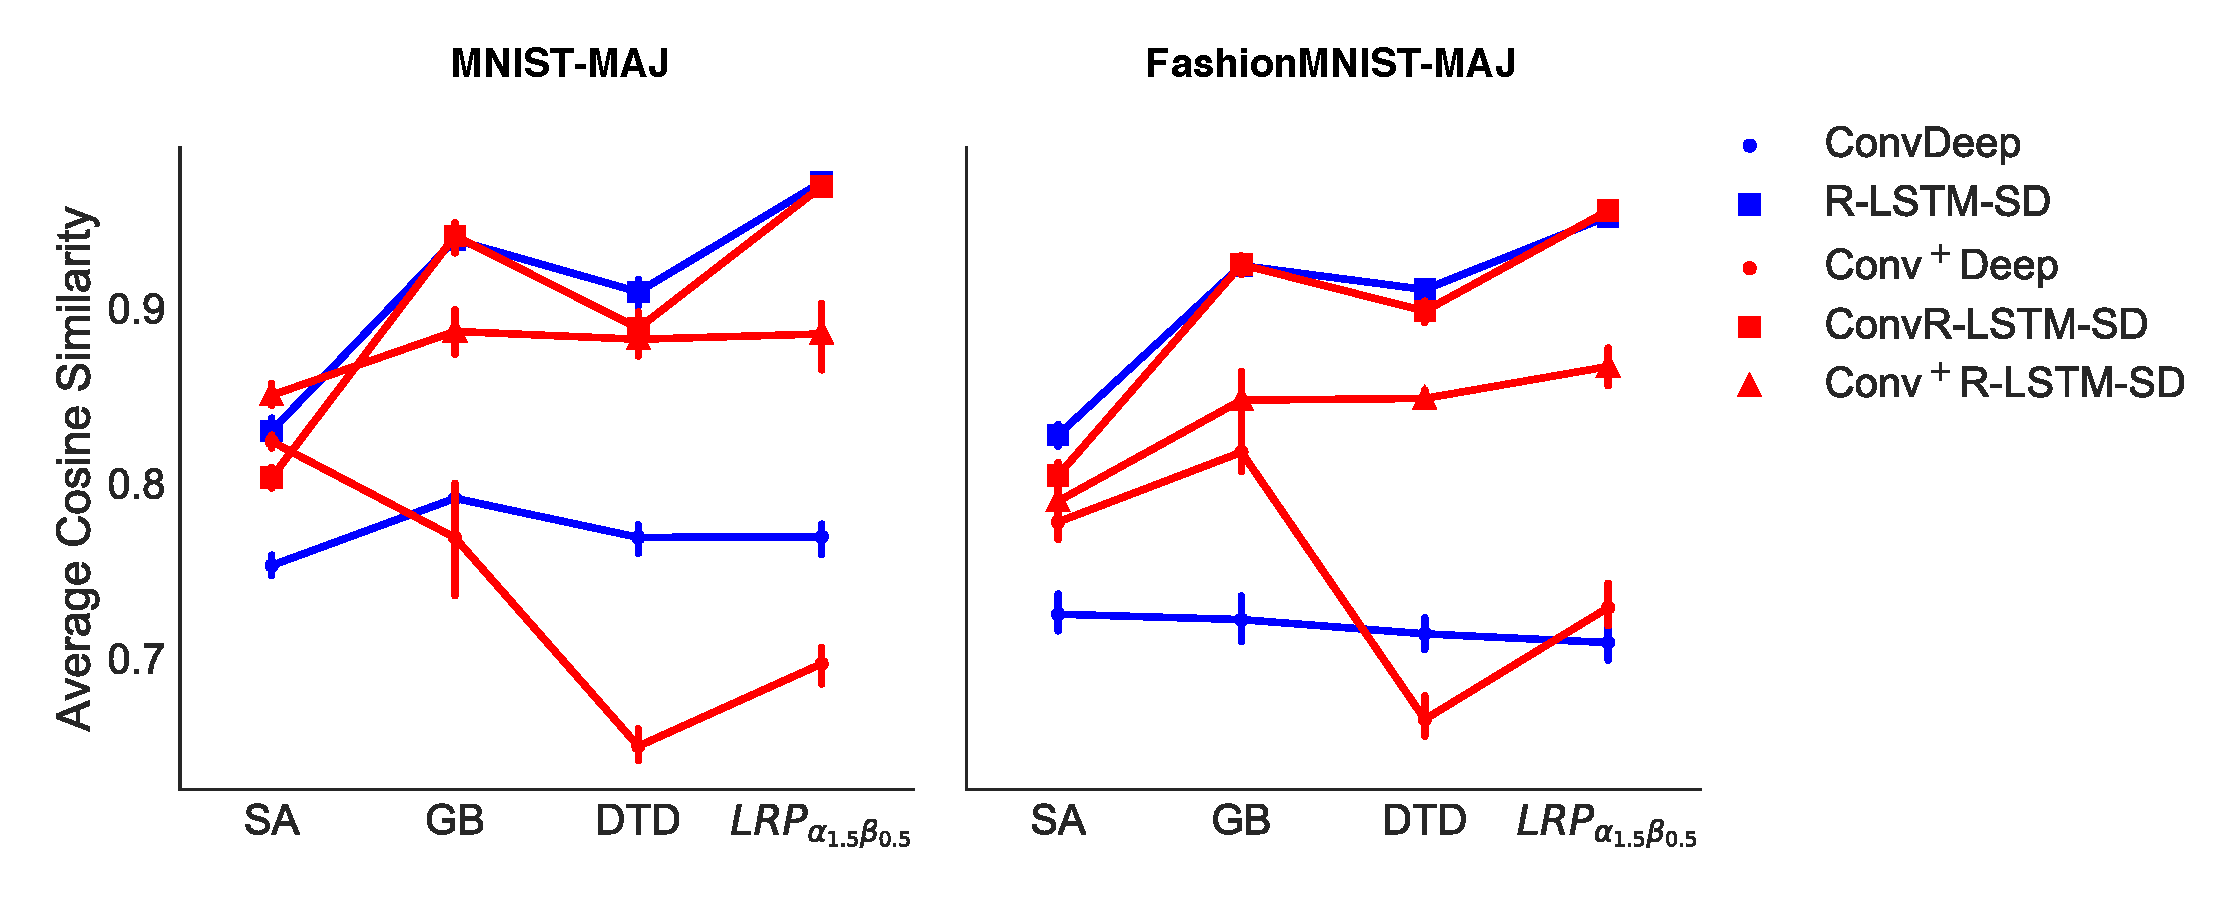
\includegraphics[width=\textwidth]{sketch/rel_dist_convdeep_trans_exp}
\patcaption{Average cosine similarity from different explanation techniques and variants of ConvDeep and R-LSTM architecture.}{The values are averaged from cross-validation results and the vertical lines depicted 95\% confidence interval. The baseline are the Deep and R-LSTM-SD architecture represented in blue. Accuracy of the models can be found at Appendix \ref{annex:model_acc}.} 
\label{fig:rel_dist_convdeep_trans_exp}
\end{figure}

\addfigure{\ref{fig:rel_dist_convdeep_trans_exp}} presents the cosine similarity measurement of this second half. Here, ConvDeep and R-LSTM-SD are the same as the previous experiments. These two architectures are presented here as the baseline presented in blue. Unexpectedly, Conv$^+$R-LSTM-SD has considerably lower the explanation capability than ConvR-LSTM-SD. On the other hand,  employing lateral connections in ConvDeep shows inconsistent influence between MNIST-MAJ and FashionMNIST-MAJ. 

 Although,  as shown in \addfigure{\ref{fig:heatmap_msc_convrlstm_pos_rel}}, explanations from ConvR-LSTM-SD are less noisy and contain more informative signal corresponding to the input, the average cosine similarity of R-LSTM-SD and ConvR-LSTM-SD look almost identical. We argue that this is a shortcoming of our quantitative measurement because the calculation of cosine similarity only considers aggregated relevance quantities and does not take smoothness and pixel-wise selectivity of explanation into account.
 
% \todo{hypo: In fact, using Tukey HSD test shows that the improvement is not statistically significant} 
%\todo{hypothesis testing}

%\clearpage

\subsection{Summary}
We have proposed several improvements to improve the explainability of RNN models and discussed their results.  Some of which show notable improvements from what we have seen in Section \ref{sec:exp2}. More precisely, employing gating unit and stationary dropout increase explainability of RNN significantly regardless of the explanation techniques.

Moreover, convolutional and pooling layers enable the models to produce more understandable explanations than traditional fully-connected layers, although this improvement does not seem to be  captured by our cosine similarity measurement. This poses a possible future work in the direction of benchmarking the quality of explanation.

Lastly, lateral connections do not show any consistent improvement for the settings we are considering. In fact, having wider confidence interval on \addfigure{\ref{fig:rel_dist_convdeep_trans_exp}} suggests that the connections seem to make the training process less stable.
